
\documentclass[final,hyperref={pdfpagelabels=false},16pt]{beamer}
\usetheme{Berlin}
\usefonttheme{professionalfonts} % using non standard fonts for beamer
\usefonttheme{serif} % default family is serif

\usepackage[russian]{babel}
\usepackage[utf8]{inputenc}
\usepackage[orientation=portrait,size=a0,scale=1,debug]{beamerposter}
\usepackage
	{
		% Дополнения Американского математического общества (AMS)
		amssymb,
		amsfonts,
		amsmath,
		amsthm,
		physics,
		graphicx
		}
\setbeamertemplate{navigation symbols}{} % минус навигация
\setbeamercolor{block body}{bg=white}
\setbeamerfont{block title}{series=\bfseries}
\let\Tiny=\tiny % решает проблему со шрифтами в TexLive
\setbeamertemplate{headline}{
	\leavevmode
	\begin{beamercolorbox}[wd=\paperwidth]{headline}
		\vspace{2ex}\\
		\begin{columns}[c]
			\begin{column}{.09\paperwidth}
			\end{column}
			\begin{column}{.675\paperwidth}
				\raggedleft
				\usebeamercolor{title in headline}{\textbf{\Huge{\inserttitle}}\\[1ex]}
				\usebeamercolor{author in headline}{\large{\insertauthor}\\[1ex]}
				\usebeamercolor{institute in headline}{\small{\insertinstitute}\\[1ex]}
			\end{column}
			\begin{column}{.25\paperwidth}
				\begin{center}
                    \begin{minipage}{0.49\linewidth}
                        
\includegraphics[width=\textwidth, keepaspectratio]{rf3}
                        
                    \end{minipage}
                    \begin{minipage}{0.49\linewidth}
                        
\includegraphics[width=\textwidth, keepaspectratio]{iap}
                        
                    \end{minipage}

                    \hfill
				\end{center}
			\end{column}
			\begin{column}{.03\paperwidth}
			\end{column}
		\end{columns}
		\vspace{2ex}\\
	\end{beamercolorbox}

 	\begin{beamercolorbox}[wd=\paperwidth]{lower separation line head}
		\rule{0pt}{2pt}
	\end{beamercolorbox}
	\vskip-2cm
	}

\setbeamertemplate{footline}{
	\begin{beamercolorbox}[wd=\paperwidth]{upper separation line foot}
		\rule{0pt}{2pt}
	\end{beamercolorbox}
	\leavevmode%
	\begin{beamercolorbox}[ht=4ex,leftskip=1cm,rightskip=1cm]{author in head/foot}%
		{Оформлено при помощи издательской системы \LaTeX}
        \hfill
		\today
		\hfill
        Github: {github.com/kannab98},   Email: {ponur0kirill@gmail.com}
		\vskip1ex
	\end{beamercolorbox}
	\vskip0pt%
	\begin{beamercolorbox}[wd=\paperwidth]{lower separation line foot}
		\rule{0pt}{2pt}
	\end{beamercolorbox}
	}

\title{Численное моделирование морской поверхности}
\author{Понур К.А.$^{1}$, Караев В.Ю.$^2$, Рябкова М.С.$^2$}
\institute{$^{1}$ Нижегородский Государственный Университет им. М.Ю. Лобачевского \\
          $^2$ Институт Прикладной Физики Российской Академии Наук}
\date{\today}
\newcommand{\tK}{\widetilde{K}}
\usepackage{mathtools}
\mathtoolsset{showonlyrefs}
\newcommand{\mean}[1]{\langle #1 \rangle}
\begin{document}
  \begin{frame}[t]{} 
    \begin{columns}[t]
      \begin{column}{.48\linewidth}
        \begin{block}{Введение}
            Для изучения и мониторинга состояния морской поверхности активно используются радиолокаторы. 
            Благодаря орбитальным скаттерометрам измеряется поле приводного ветра в Мировом океане, радиовысотомеры измеряют высоту значительного волнения и средний уровень
            морской поверхности. Для обнаружения разливов нефти и нефтепродуктов активно используются радиолокаторы с синтезированной апертурой.

            Современные достижения в радиолокационном зондировании базируются на результатах исследования рассеяния электромагнитных волн морской поверхностью. Тем не менее, остается ряд нерешенных 
            вопросов по моделям рассеяния. Также, существующие радиолокационные системы не всегда позволяют получить необходимую информацию о состоянии приповерхностного слоя океана, что обуславливает необходимость совершенствования измерительной аппаратуры. 

            На этапе поиска оптимальной схемы измерения необходимо оценить вклад в спектральные и энергетические характеристики отраженного сигнала параметров волнения, течений, поверхностных пленок. Численное моделирование является мощным инструментом, позволяющим решать эти задачи.
        \end{block}
        \begin{block}{Моделирование}
            Рассмотрим задачу моделирования морской поверхности по заданному спектру волнения.

            Спектр двумерного волнения представим в виде функции с разделяющимися переменными (см. рис. \ref{fig:spec}):
        \begin{equation}
            \label{eq:}
            S(\vec k) = S(k) \Phi(\phi), ~ k = \sqrt{k_x^2+k_y^2},~ \phi=\arctg{\frac{k_x}{k_y}},\quad \int\limits_{-\pi}^{\pi} \Phi(\phi) \dd{\phi} = 1.
        \end{equation}
        
            Поверхность представим как сумму гармоник с детерменированными амплитудами и случайными фазами
        \begin{equation}
            \zeta(\vec r, t)= \sum\limits_{n=1}^N \sum_{m=1}^M A_n(k_n)\cdot 
            \Phi_{nm}(\phi_m) \cos(\omega_n t + \vec k_n \vec r + \psi_{nm}),
        \end{equation}
        Амплитуда, которая является мощностью на интервале $\Delta k_n$, вычисляется по спектру моделируемой поверхности
        \begin{equation}
            A_n(k_n)=\sqrt{ \int\limits_{(\Delta k_n)}  2 S(k) \dd{k}}
        \end{equation}
        $\Phi_{nm}$ -- азимутальное распределение, вычисляемое следующим образом:
        \begin{equation}
        \Phi_{nm}(k_n,\phi_m)=\sqrt{\Phi(k_n,\phi_m) \Delta \phi},
        \end{equation}
        $\Delta \phi$ -- шаг по углу
        \begin{figure}[h]
            \begin{minipage}{0.24\linewidth}
                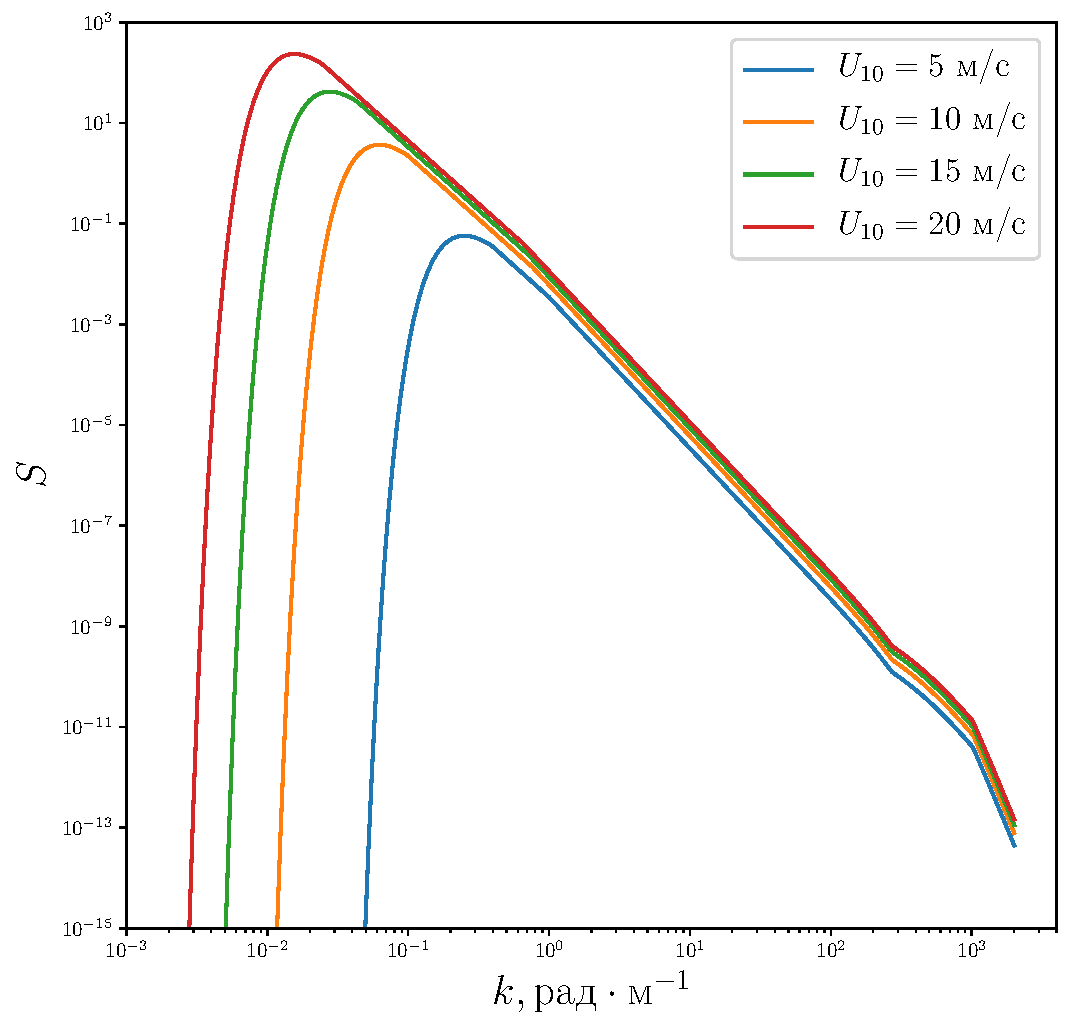
\includegraphics[width=\linewidth]{fig/full_spectrum1}
                \centering
                (a)
            \end{minipage}
            \begin{minipage}{0.24\linewidth}
                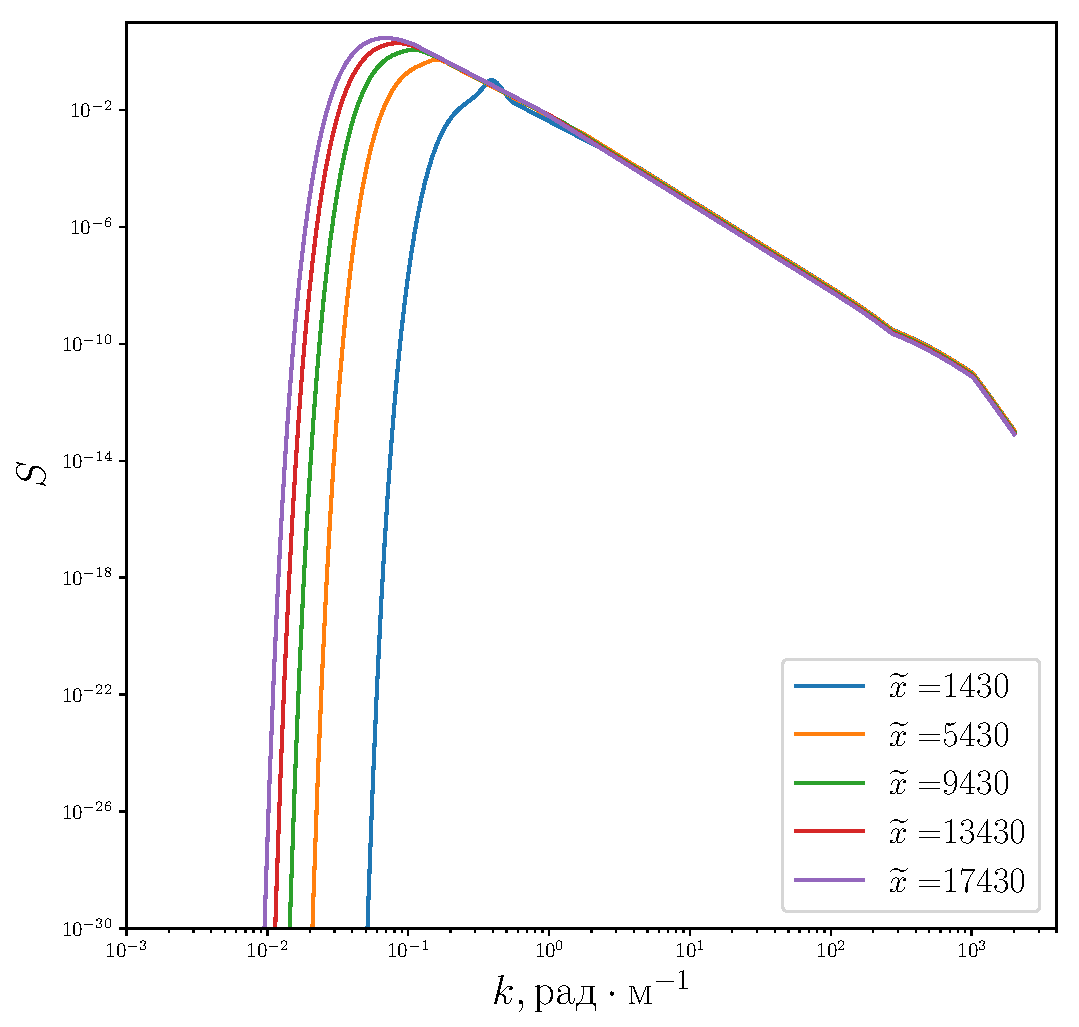
\includegraphics[width=\linewidth]{fig/full_spectrum2}
                \centering
                (b)
            \end{minipage}
            \begin{minipage}{0.24\linewidth}
                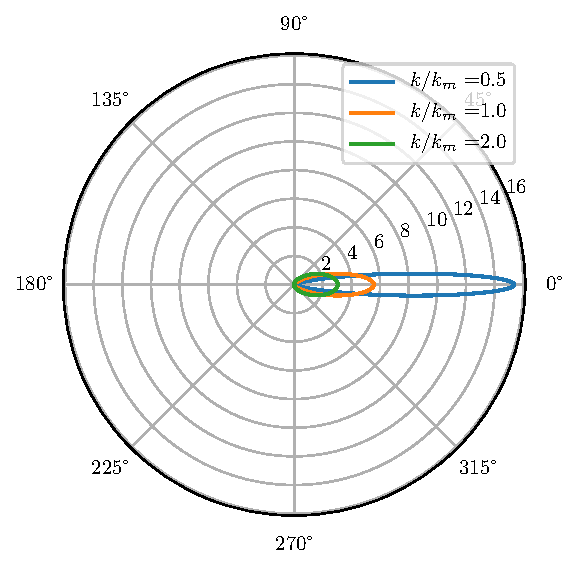
\includegraphics[width=\linewidth]{fig/full_angles1}
                \centering
                (c)
            \end{minipage}
            \begin{minipage}{0.24\linewidth}
                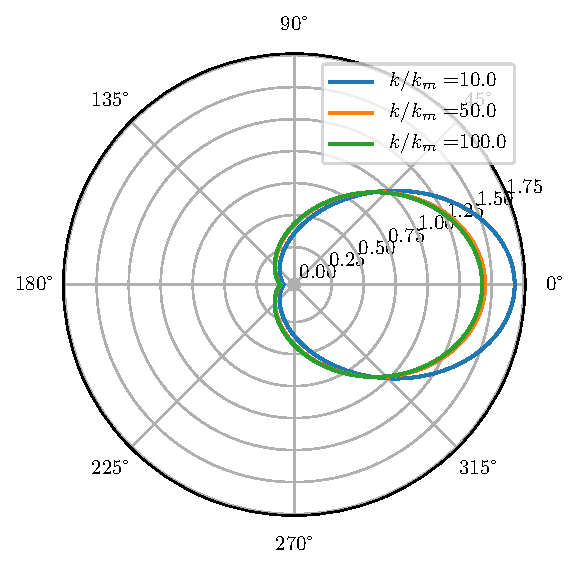
\includegraphics[width=\linewidth]{fig/full_angles2}
                \centering
                (d)
            \end{minipage}
            \label{fig:spec}
            \caption{(a) Спектр высот $S(k)$ при фиксированном значении  $\tilde x = 20170$ и меняющейся скорости ветра 
            (b) Спектр высот $S(k)$ при фиксированном значении скорости ветра $U_{10} = 10 \frac{\text{м}}{\text{с}}$ и меняющемся разгоне 
        (c,d) Угловое распределение  $\Phi_k(\phi)$ в полярных координатах для разных значений соотношений  $\frac{k}{k_m}$, где $k_m$ - координата пика спектра $S(k)$ при фиксированной скорости ветра}
        \end{figure}
        \begin{figure}[h]
            \begin{minipage}{0.45\linewidth}
                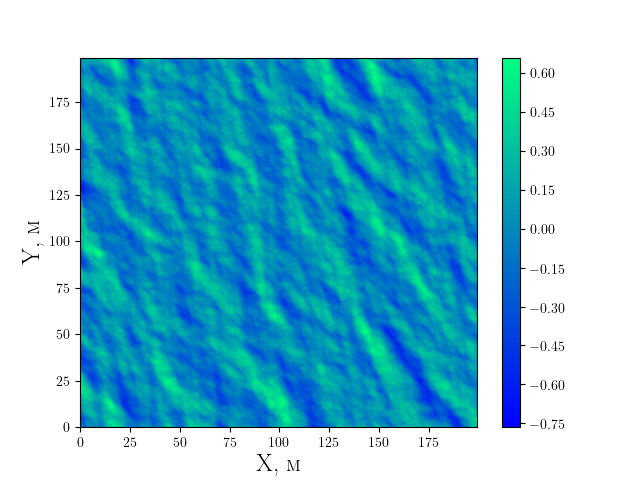
\includegraphics[width=\linewidth]{fig/water5.png}
                \centering
                (a)
            \end{minipage}
            \begin{minipage}{0.45\linewidth}
                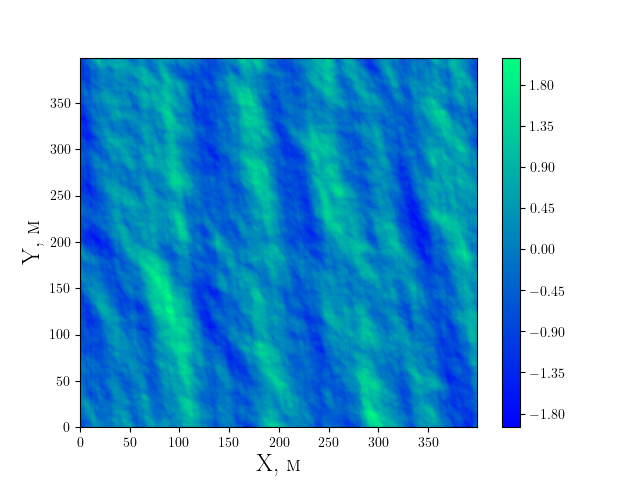
\includegraphics[width=\linewidth]{fig/water10}
                \centering
                (b)
            \end{minipage}
            \caption{Пример смоделированной поверхности при разной скорости и направлении ветра (a) $U_{10} = 5 \text{ м/с }$, (b) $U_{10} = 10 \text{ м/с}$}
        \end{figure}
        \end{block}
        \begin{block}{<<Choppy wave>> model}
            На практике, волна имеет не синусоидальную форму, а несколько заостренную, поэтому при моделировании необходимо учесть этот эффект.
            %Для этого к стандартному подходу моделирования применялась модикация:  чоппи вав модел. 
            Модель заключается в нелинейном преобразовании координат
            \begin{gather}
                x = x_{0} - \sum\limits_{n=1}^N \sum_{m=1}^M \frac{\vec k_n}{\abs{\vec k_n}} \vec x_0 A_n(k_n)\cdot 
            \Phi_{nm}(\phi_m) \sin(\omega_n t + \vec k_n \vec r_0 + \psi_{nm}),\\
                y = y_{0} - \sum\limits_{n=1}^N \sum_{m=1}^M \frac{\vec k_n}{\abs{\vec k_n}} \vec y_0 A_n(k_n)\cdot 
            \Phi_{nm}(\phi_m) \sin(\omega_n t + \vec k_n \vec r_0 + \psi_{nm}),\\
            \zeta(\vec r, t)= \sum\limits_{n=1}^N \sum_{m=1}^M A_n(k_n)\cdot 
            \Phi_{nm}(\phi_m) \cos(\omega_n t + \vec k_n \vec r_0 + \psi_{nm}).
            \end{gather}
            Зная исходный спектр волнения мы можем посчитать все статистические характеристики нового процесса
            \begin{gather}
                \mean{\tilde \zeta} =  - \sigma_1^2, \quad \mean{\tilde \zeta^2} = \sigma_0^2 - 2\Sigma_1\\
                \mean{\tilde \zeta^3} = -3 \sigma_0^2 \sigma_1^2, \quad \mean{\tilde \zeta^4} = 3 \sigma_0^4 
                \qty(1- 4 \frac{\Sigma_{1}}{\sigma_0^2}), \text{ где}
            \end{gather}
            \begin{gather}
                \sigma^2_{\alpha \beta } = \int \frac{{k_x}^\alpha {k_y}^{\beta}}{\qty(\sqrt{k_x^2+k_y^2})}S(\vec k) \dd{\vec k}, \quad
                \sigma_n^2 = \int k^n S(\vec k) \dd{\vec k},\quad \Sigma_1 = \sigma_{11}^4 - \sigma_{20}^2 \sigma_{02}^2
            \end{gather}
            \begin{figure}[h]
                    \centering
                    \begin{minipage}{0.45\linewidth}
                        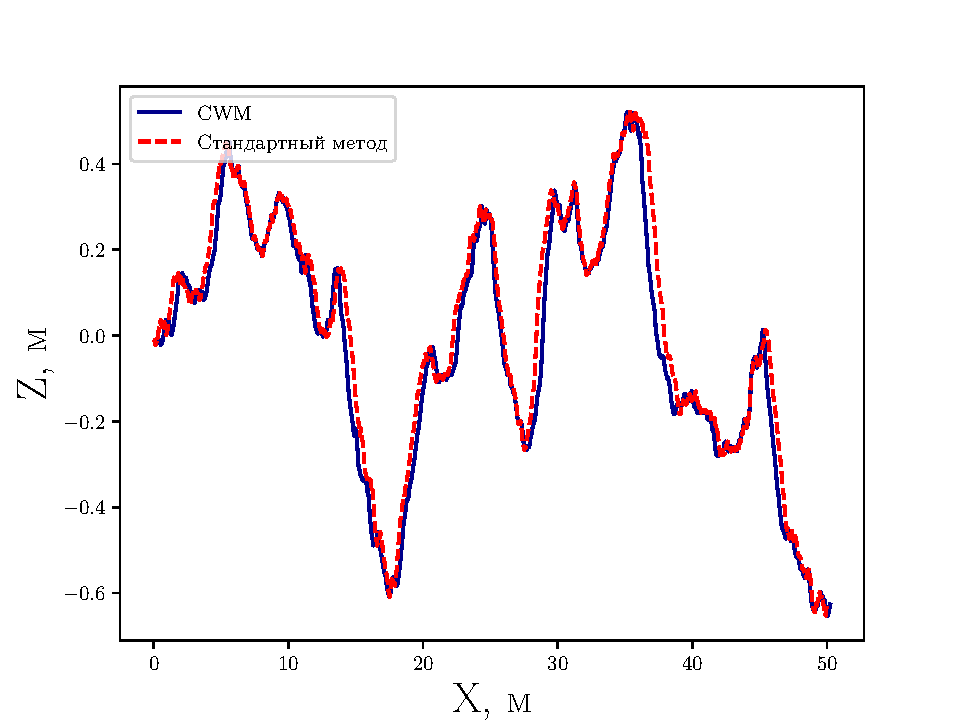
\includegraphics[width=\linewidth]{fig/cwm}
                        \centering 
                        (a)
                    \end{minipage}
                    \begin{minipage}{0.45\linewidth}
                        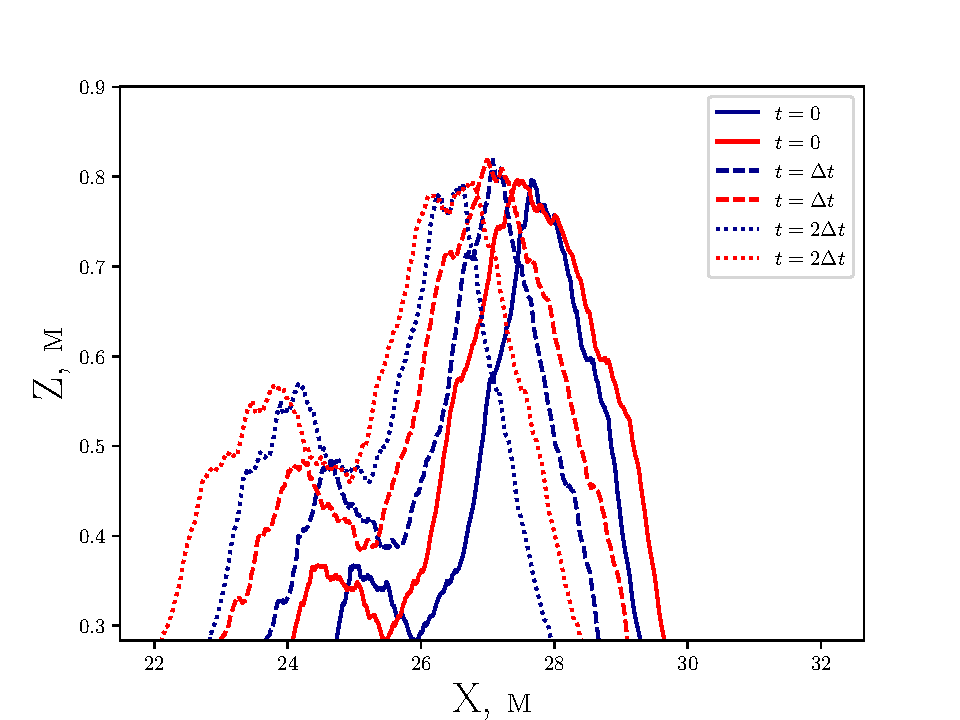
\includegraphics[width=\linewidth]{fig/evolution}
                        \centering
                        (b)
                    \end{minipage}
                    \caption{(a) сравнение двух систем  (b) эволюция <<линейной>>  и  <<нелинейной>>  систем, $\Delta t = 0.2 \text{ с}$}
                    \label{fig:}
                \end{figure}


        \end{block}
        
      \end{column}
      \begin{column}{.48\linewidth}
        \begin{block}{Метод <<отбеливания>> спектра}
            Предположим, что гармонические составляющие при больших $\rho=r_{2}-r_{1}$ складываются <<некогерентным>> образом. То есть  мощность шума определяется как
            \begin{equation}
                \sigma^2_{\text{шум}}= \sum_{i=1}^N \frac{b_i^2}{2}
            \end{equation}
            В области малых $\rho$ гармоники суммируются <<когерентно>> и соответствующая мощность равна
            \begin{equation}
                \tK^2(0)=\qty(\sum_{i=1}^N b_i)^2
            \end{equation}
            Введем функцию, характеризующую относительную мощность шумов
            \begin{equation}
                \label{eq:Q}
                Q = \frac{\sigma^2_{\text{шум}}}{\tK^2(0)}
            \end{equation}
            Минимизируем величину \eqref{eq:Q}, решая систему уравнений
            \begin{equation}
                \label{eq:cases}
                \pdv{Q}{b_i}=\frac{b_i}{\qty (\sum\limits_{j=1}^{N} b_j)^2} - \frac{\sum\limits_{j=1}^{N} b_j^2}{\qty (\sum\limits_{j=1}^{N} b_j)^3}, ~ i = 1\hdots N.
            \end{equation}
            Она сводится к следующей системе:  $b_i \sum\limits_{j=1}^{N} b_j -\sum\limits_{j=1}^{N} b_j^2=0 $
             \vfill
            Частным решением этой системы является $b_1=b_2=\hdots=b_N$.
            \vfill
           \begin{equation}
                \text{Для высот:}\quad 	b_i=b_1= \frac{K(0)}{N}=\frac1N \int\limits_0^{\infty} S(k) \dd{k}
           \end{equation}
           \begin{equation}
                \text{Для наклонов:}\quad 	b^{\theta}_i=b^{\theta}_1= \frac{K^{\theta}(0)}{N}=\frac1N \int\limits_0^{\infty} k^2S(k) \dd{k}
           \end{equation}
            Потребуем сопряжения в нуле всех производных  функций
            $\tK(\rho)$ и $K(\rho)$. 
            Для функции корреляции стационарной случайной функции $K(\rho)$ справедливо
            \begin{equation}
                K'_{\rho}=\pdv[2]{K(\rho)}{\rho}=\int\limits_{0}^{\infty} k^2 S(k)\cos(k \rho)\dd{k}
            \end{equation}
            А значит можно переписать наше требование в виде
            \begin{equation}
                \sum_{i=1}^N b_i k_i^{2p}=\int\limits_{0}^{\infty} k^{2p}S(k)\dd{k}, p = 1,2,\dots,N.
            \end{equation}
            Решать такую систему довольно сложно, поэтому потребуем выполнение более простого равенства
            \begin{equation}
                \sum_{i=1}^N b_ik_i^{2}=\int\limits_{0}^{\infty} k^{2}S(k)\dd{k}
            \end{equation}
            \begin{minipage}{0.49\linewidth}
                \centering Для наклонов:
                \begin{equation}
                    k_i=\sqrt\frac{N}{{\int\limits_{0}^{\infty} k^2 S(k) \dd{k}}}\cdot {\int\limits_{\Delta k_i} k^4 S(k) \dd{k}}
                \end{equation}
                \end{minipage}
                \hfill
                \begin{minipage}{0.49\linewidth}
                \centering Для высот:
                \begin{equation}
                    k_i=\sqrt\frac{N}{{\int\limits_{0}^{\infty} S(k) \dd{k}}}\cdot \int\limits_{\Delta k_i} k^2 S(k) \dd{k}
                \end{equation}
                \end{minipage}
                \vfill
                Решением будем считать суперпозицию решения системы уравнений
                \eqref{eq:cases} для высот и наклонов.

                Точность моделирования будем определять близостью корреляционной функции реального волнения $K(\rho)$ с корреляционной функцией модельного $\widetilde K(\rho)$. 
                \begin{equation}
                    \label{eq:}
                    \eta = \norm{K(\rho) - \widetilde K(\rho)} = \sqrt{\sum\limits_i {\qty( K(\rho_i) - \widetilde K(\rho_i) )^2}}  
                \end{equation}
                Сравним значения $\eta$ для логарифмического разбиения частотной плоскости $\eta_0$ и для метода отбеливания спектра $\eta_1$.

                \begin{center}
                    
                \begin{tabular}{|c|c|c|c|c|c|}
                    $\eta_0^{\text{в}}$ & $\eta_0^{\text{н}}$ & $\eta_1^{\text{н}}$ & $\eta_1^{\text{в}}$ & $\eta_1^{\text{н}}/\eta_0^{\text{н}}$ & $\eta_1^{\text{н}}/\eta_0^{\text{н}}$ \\ [0.5ex]

                \hline 
                    0.018 & 0.056 & 0.007 & 0.049 & 0.4 & 0.86
             \end{tabular}
                \end{center}
                \begin{figure}[H]
                    \begin{minipage}{0.32\linewidth}
                            \centering
                            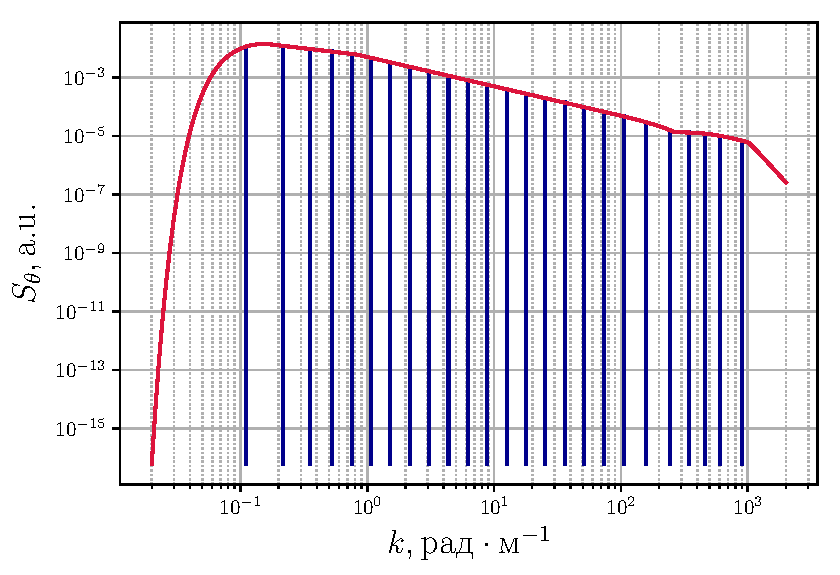
\includegraphics[width=\linewidth]{fig/split_angles}	
                    \end{minipage}
                    \hfill
                    \begin{minipage}{0.32\linewidth}
                            \centering
                            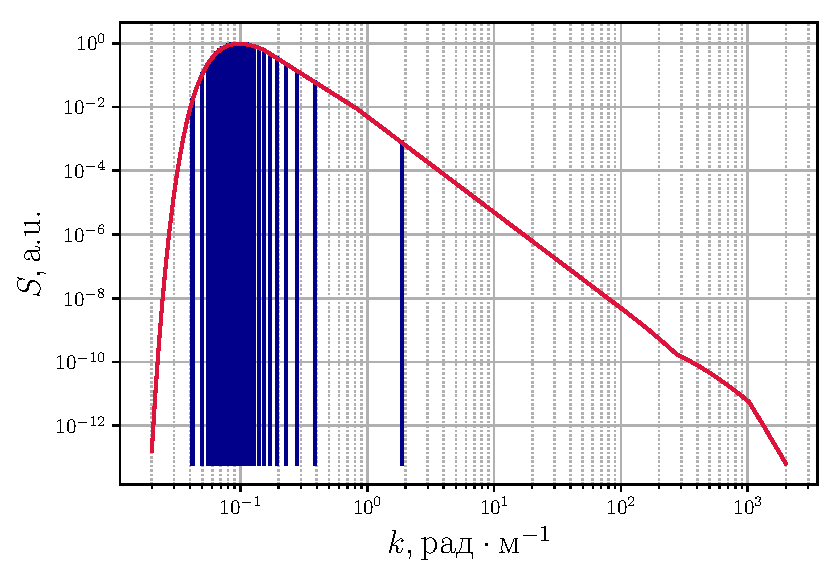
\includegraphics[width=\linewidth]{fig/split_height}
                    \end{minipage}
                    \begin{minipage}{0.32\linewidth}
                            \centering
                    \vspace{-15pt}
                            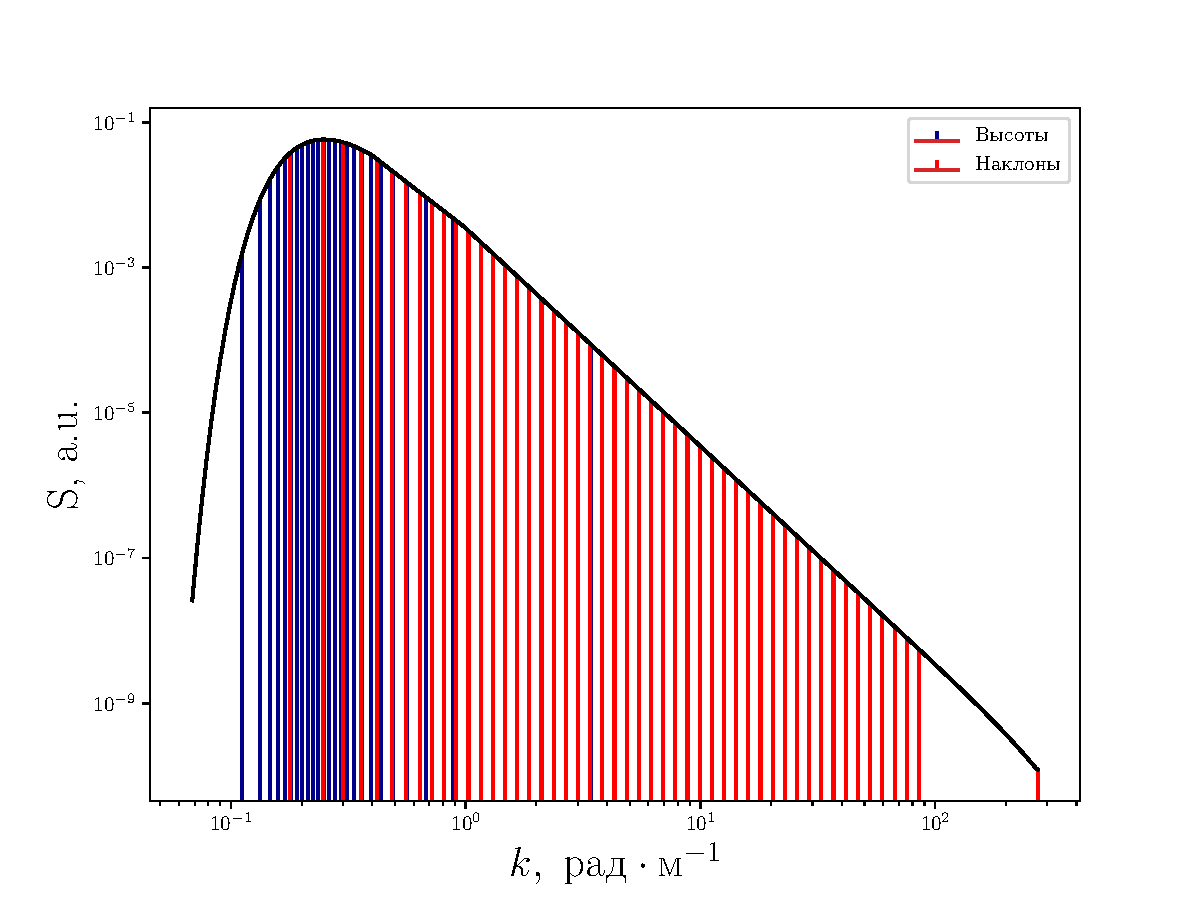
\includegraphics[width=\linewidth]{nodes}
                    \end{minipage}
                    \caption{Расположении узлов по методу <<отбеливания>> спектра  для (a) наклонов и (b) высот соответственно. $U=10 \frac{\text{м}}{c}$, $N=25$; (c) суперпозиция 
                    метода <<отбеливания>> для высот и наклонов}
                    \label{fig:splits}		
                \end{figure}
                \begin{figure}[h]
                    \centering
                    \begin{minipage}{0.49\linewidth}
                            \centering
                            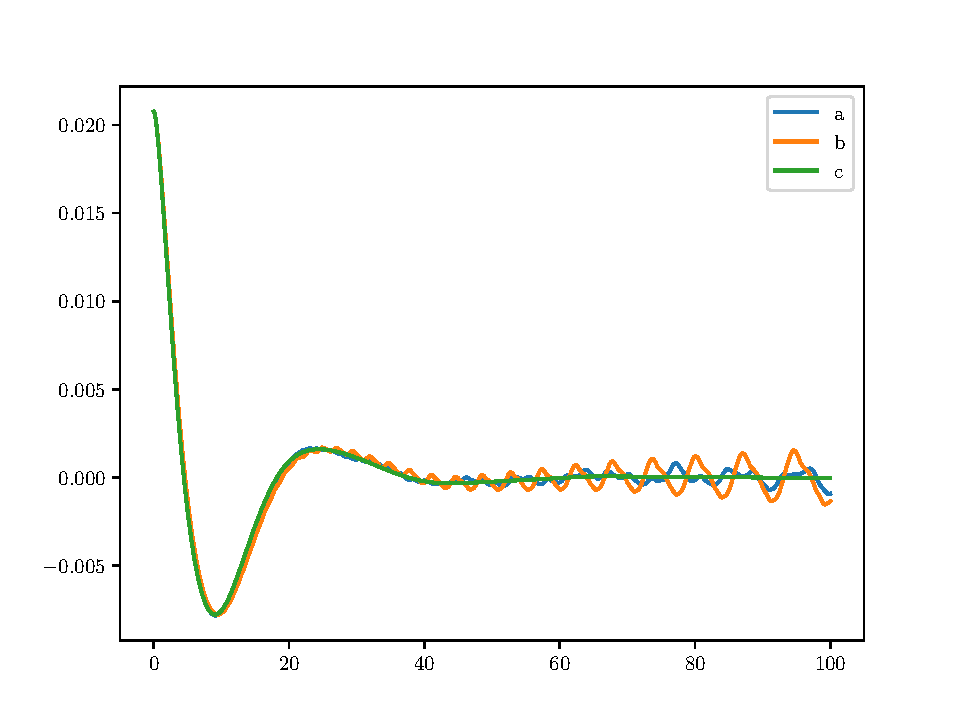
\includegraphics[width=\linewidth]{fig/corr1}

                            (a)
                    \end{minipage}
                    \begin{minipage}{0.49\linewidth}
                            \centering
                            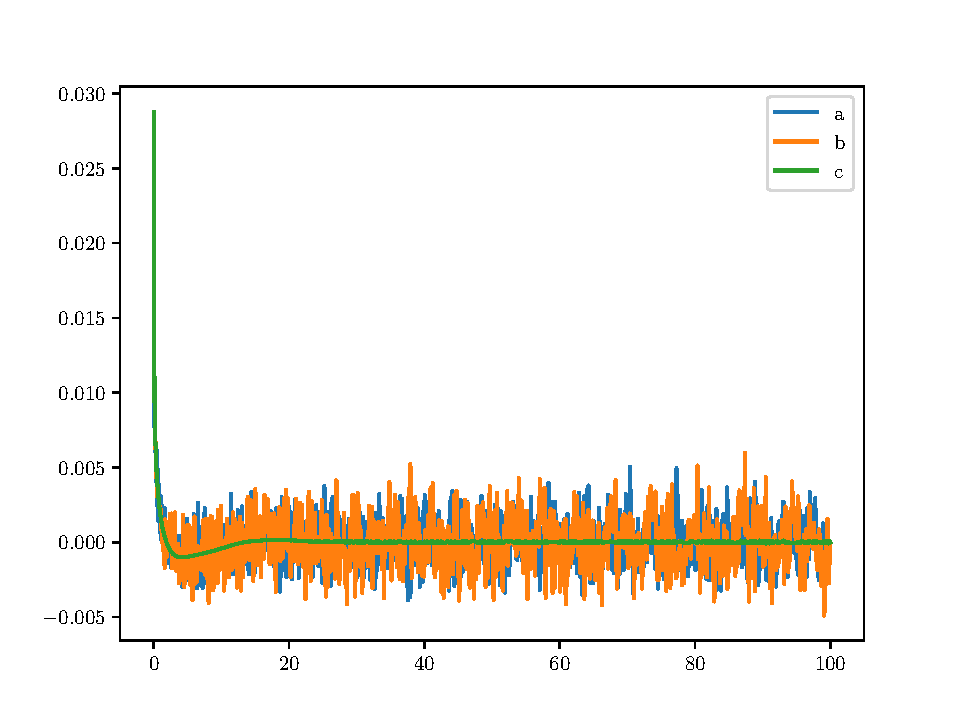
\includegraphics[width=\linewidth]{fig/corr2}

                            (b)
                    \end{minipage}
                    \caption{Корреляционные функции высот и уклонов  при различных расположениях гармоник. $U=5\frac{\text{м}}{\text{с}},~ N = 128$; 
                    (a) расположение по методу <<отбеливания>> спектра, 
                    (b) логарифмическое расположение;
                    (c) теоретическая корреляционная функция }
                    \label{fig:}
                \end{figure}
        \end{block}
        \begin{block}{Заключение}
            \small
            В данной работе была произведена оптимизация разбиения частотной плоскости на участки, что позволило добиться увеличения точности моделирования при сохранении количества спектральных компонент.

Однако, смоделированная с помощью суммы синусоид поверхность будет отличаться от морской поверхности, так как реальная волна имеет заостренную и ассиметричную форму.  Поэтому кроме «линейной» поверхности в ходе исследования моделировалась «нелинейная» поверхность.
Для этого использовался подход, предложенный в \cite{CWM}, что позволило обострить гребни волн.  Нелинейная поверхность будет использоваться для проведения «численных» экспериментов с радиолокаторами, что повысит достоверность модельных оценок.


Задача, которую планируется рассмотреть в ходе дальнейших исследований, связана с моделированием асимметричных волн.
        \end{block}
        \begin{block}{Литература}
            \footnotesize
            \begin{thebibliography}{}
                \bibitem{Karaev1} \textit{В.Ю.Караев, М.Б. Каневский, Г.Н. Баландина}, Численное моделирование поверхностного волнения и дистанционное зондирование // Препринт №552 ИПФ РАН, 2002, С.1-10.
                \bibitem{Veber} \textit{В.Л. Вебер}, О моделировании случайного профиля морской поверхности // Изв. вузов. Радиофизика. 2017. Т. 60, № 4. С. 346.
                \bibitem{CWM} F. Nouguier, <<Choppy wave>> model for nonlinear gravity waves // Journal of Geophysical Research, v.114, 2009, p. 1-16
                \bibitem{Ryabkova} M.Rybkova, V.Karaev, J.Guo and Yu. Tichenko, "A Review 
                of Wave Spectrum Models as Applied to the Problem of Radar Probing 
                of the Sea Surface" // Journal of Geophysical Research: Oceans
            \end{thebibliography}
        \end{block}
      \end{column}
    \end{columns}
  \end{frame}
\end{document}
